

\begin{table}[h]
    \centering
    \caption{Comparação do Tempo do Insertion Sort}
    \begin{tabular}{|c|c|c|c|c|c|c|}
        \hline
        Tamanho de Entrada & 10 & 100 & 1000 & 10000 & 100000 & 1000000 \\
        \hline
        Crescente & 0.000000 & 0.000000 & 0.000000 & 0.000000 & 0.000000 & 0.003000 \\
        \hline
        Decrescente & 0.000000 & 0.000000 & 0.001000 & 0.111000 & 10.856000 & 1088.031000 \\
        \hline
        Aleatória & 0.000000 & 0.000000 & 0.001000 & 0.056000 & 5.439000 & 547.712000 \\
        \hline
    \end{tabular}
    \label{tab:comparacao}
\end{table}
Para a elaboração da tabela (Tabela \ref{tab:comparacao}) e do gráfico (Figura \ref{grafico_insert}), foi escrito um algoritmo em C para gerar arquivos com tamanhos de entrada n = 10, 100, 1.000, 10.000, 100.000 ou 1.000.000 formados por uma sequência de numeros aleatóios  e seus ”n” sucessores. Podem ser gerados em ordem Crescente, Decrescente ou Aleatória. Os resultados mostram que o Insertion Sort performa excepcionalmente bem em conjuntos
de dados pequenos e em situações onde a entrada já está parcialmente ordenada. Entretanto,
seu desempenho degrada significativamente para entradas maiores e particularmente para o
caso em que os dados estão ordenados de forma decrescente. Nestes cenários, o algoritmo
exibe um comportamento quadrático, tornando-o impraticável para conjuntos de dados muito
grandes.

 \begin{figure}[htbp]
    \centering
    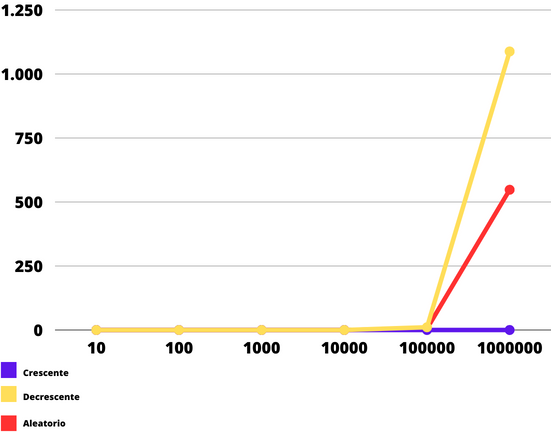
\includegraphics[width = 10cm]{Imagens/Insertion Sort/graficocanvas.png}
    \caption{Gráfico de tempo do algoritmo Inserion Sort. }
    \label{grafico_insert}
\end{figure}



